\documentclass{article}
\usepackage{pgfplots}
\usepackage{amssymb, amsmath}
\usepackage{tikz}
\usepackage{xcolor}
\pgfplotsset{compat=1.7}






\begin{document}
\pgfmathdeclarefunction{gauss}{2}{\pgfmathparse{1/(#2*sqrt(2*pi))*exp(-((x-#1)^2)/(2*#2^2))}%
}
\begin{tikzpicture}
\begin{axis}[no markers, domain=0:10, samples=100,
axis lines*=left, xlabel=Standard deviations, ylabel=Frequency,,
height=6cm, width=10cm,
xtick={-3, -2, -1, 0, 1, 2, 3}, ytick=\empty,
enlargelimits=false, clip=false, axis on top,
grid = major]
\addplot [fill=cyan!20, draw=none, domain=-3:3] {gauss(0,1)} \closedcycle;
\addplot [fill=orange!20, draw=none, domain=-3:-2] {gauss(0,1)} \closedcycle;
\addplot [fill=orange!20, draw=none, domain=2:3] {gauss(0,1)} \closedcycle;
\addplot [fill=blue!20, draw=none, domain=-2:-1] {gauss(0,1)} \closedcycle;
\addplot [fill=blue!20, draw=none, domain=1:2] {gauss(0,1)} \closedcycle;
\addplot[] coordinates {(-1,0.4) (1,0.4)};
\addplot[] coordinates {(-2,0.3) (2,0.3)};
\addplot[] coordinates {(-3,0.2) (3,0.2)};
\node[coordinate, pin={68.2\%}] at (axis cs: 0, 0.4){};
\node[coordinate, pin={95\%}] at (axis cs: 0, 0.3){};
\node[coordinate, pin={99.7\%}] at (axis cs: 0, 0.2){};
\node[coordinate, pin={34.1\%}] at (axis cs: -0.5, 0){};
\node[coordinate, pin={34.1\%}] at (axis cs: 0.5, 0){};
\node[coordinate, pin={13.6\%}] at (axis cs: 1.5, 0){};
\node[coordinate, pin={13.6\%}] at (axis cs: -1.5, 0){};
\node[coordinate, pin={2.1\%}] at (axis cs: 2.5, 0){};
\node[coordinate, pin={2.1\%}] at (axis cs: -2.5, 0){};
\end{axis}
\end{tikzpicture}



\begin{tikzpicture}
\begin{axis}[every axis plot post/.append style={
  mark=none,domain=-2:4.5,samples=500,smooth}, % All plots: from -2:2, 50 samples, smooth, no marks
  axis x line*=bottom, % no box around the plot, only x and y axis
  axis y line*=left, % the * suppresses the arrow tips
  enlargelimits=upper] % extend the axes a bit to the right and top
  \addplot {gauss(0,0.5)};
  \addplot {gauss(1,0.75)};
  \addplot {gauss(1.5,1.25)};
\end{axis}
\end{tikzpicture}



\begin{tikzpicture}
\begin{axis}[every axis plot post/.append style={
  mark=none,domain=-3:3,samples=50,smooth}, % All plots: from -2:2, 50 samples, smooth, no marks
  axis x line*=bottom, % no box around the plot, only x and y axis
  axis y line*=left, % the * suppresses the arrow tips
  enlargelimits=upper] % extend the axes a bit to the right and top
  \addplot {gauss(0,1)};
  \addplot {gauss(0,0.5)};
  \addplot {gauss(0,1.5)};
\end{axis}
\end{tikzpicture}

$$\displaystyle
 f(x) = \frac{1}{\sigma\sqrt{2\pi}} 
  \exp\left( -\frac{1}{2}\left(\frac{x-\mu}{\sigma}\right)^{\!2}\,\right)$$
  
 \begin{tikzpicture}

\begin{axis}[no markers, domain=0:10, samples=100,
axis lines*=left, xlabel=Test, ylabel=axis $y$,
height=6cm, width=10cm,
xticklabels={Test A,Test B,Test C,Test D, Test A,Test B,Test C,Test D}, ytick=\empty,
enlargelimits=false, clip=false, axis on top,
grid = major]
\addplot [fill=cyan!20, draw=none, domain=-3:3] {gauss(0,1)} \closedcycle;
\addplot [fill=orange!20, draw=none, domain=-3:-2] {gauss(0,1)} \closedcycle;
\addplot [fill=orange!20, draw=none, domain=2:3] {gauss(0,1)} \closedcycle;
\addplot [fill=blue!20, draw=none, domain=-2:-1] {gauss(0,1)} \closedcycle;
\addplot [fill=blue!20, draw=none, domain=1:2] {gauss(0,1)} \closedcycle;
\end{axis}
\end{tikzpicture}


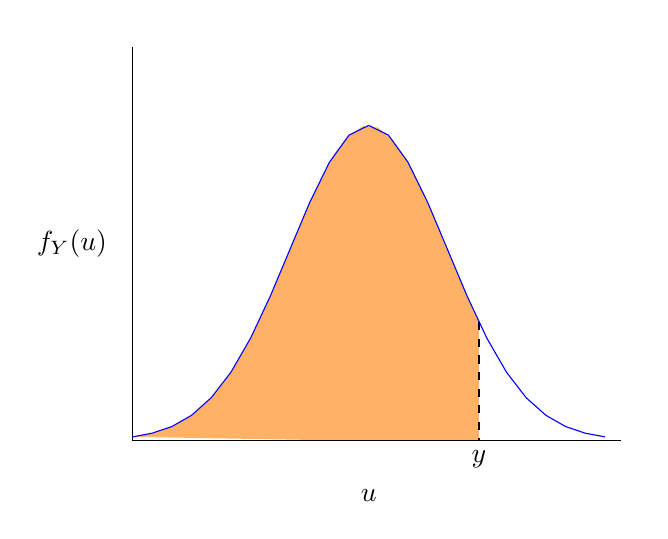
\begin{tikzpicture}
% define normal distribution function 'normaltwo'
\def\normaltwo{\x,{4*1/exp(((\x-3)^2)/2)}}

% input y parameter
\def\y{4.4}

% this line calculates f(y)
\def\fy{4*1/exp(((\y-3)^2)/2)}

% Shade orange area underneath curve.
\fill [fill=orange!60] (2.6,0) -- plot[domain=0:4.4] (\normaltwo) -- ({\y},0) -- cycle;

% Draw and label normal distribution function
\draw[color=blue,domain=0:6] plot (\normaltwo) node[right] {};

% Add dashed line dropping down from normal.
\draw[dashed] ({\y},{\fy}) -- ({\y},0) node[below] {$y$};

% Optional: Add axis labels
\draw (-.2,2.5) node[left] {$f_Y(u)$};
\draw (3,-.5) node[below] {$u$};

% Optional: Add axes
\draw[] (0,0) -- (6.2,0) node[right] {};
\draw[] (0,0) -- (0,5) node[above] {};

\end{tikzpicture}





\begin{tikzpicture}
	\begin{axis}[
	scale only axis,
	axis x line=middle,
	axis y line=middle,
	inner axis line style={=>},
	width=15cm,height=6cm,
	ymin=0,ymax=0.45,
	xmin=-3.5,xmax=3.5,
	axis line style = thick,
	ticks =none,
	every axis x label/.style={at={(current axis.right of origin)},anchor=west},
	every axis y label/.style={at={(current axis.north)},above=0.5mm},
	xlabel={$z$},
	ylabel={$f_{Z}(z)$}
	]
	\addplot [domain=-3.5:3.5,samples=500,blue,thick] {gauss(0,1)};
	\end{axis}
	\end{tikzpicture}
	
	

% latex table generated in R 3.0.1 by xtable 1.7-1 package
% Tue Oct 15 10:15:49 2013
\begin{center}
\begin{table}[ht]
\small
\centering
\begin{tabular}{rrrrrrrrrrr}
  \hline
\textbf{N(0,1)} 0 & 0.001 & 0.002 & 0.003 & 0.004 & 0.005 & 0.006 & 0.007 & 0.008 & 0.009 \\ 
  \hline
0 & 0.5000 & 0.5040 & 0.5080 & 0.5120 & 0.5160 & 0.5199 & 0.5239 & 0.5279 & 0.5319 & 0.5359 \\ 
  0.1 & 0.5398 & 0.5438 & 0.5478 & 0.5517 & 0.5557 & 0.5596 & 0.5636 & 0.5675 & 0.5714 & 0.5753 \\ 
  0.2 & 0.5793 & 0.5832 & 0.5871 & 0.5910 & 0.5948 & 0.5987 & 0.6026 & 0.6064 & 0.6103 & 0.6141 \\ 
  0.3 & 0.6179 & 0.6217 & 0.6255 & 0.6293 & 0.6331 & 0.6368 & 0.6406 & 0.6443 & 0.6480 & 0.6517 \\ 
  0.4 & 0.6554 & 0.6591 & 0.6628 & 0.6664 & 0.6700 & 0.6736 & 0.6772 & 0.6808 & 0.6844 & 0.6879 \\ 
  0.5 & 0.6915 & 0.6950 & 0.6985 & 0.7019 & 0.7054 & 0.7088 & 0.7123 & 0.7157 & 0.7190 & 0.7224 \\ 
  0.6 & 0.7257 & 0.7291 & 0.7324 & 0.7357 & 0.7389 & 0.7422 & 0.7454 & 0.7486 & 0.7517 & 0.7549 \\ 
  0.7 & 0.7580 & 0.7611 & 0.7642 & 0.7673 & 0.7704 & 0.7734 & 0.7764 & 0.7794 & 0.7823 & 0.7852 \\ 
  0.8 & 0.7881 & 0.7910 & 0.7939 & 0.7967 & 0.7995 & 0.8023 & 0.8051 & 0.8078 & 0.8106 & 0.8133 \\ 
  0.9 & 0.8159 & 0.8186 & 0.8212 & 0.8238 & 0.8264 & 0.8289 & 0.8315 & 0.8340 & 0.8365 & 0.8389 \\ 
  1 & 0.8413 & 0.8438 & 0.8461 & 0.8485 & 0.8508 & 0.8531 & 0.8554 & 0.8577 & 0.8599 & 0.8621 \\ 
  1.1 & 0.8643 & 0.8665 & 0.8686 & 0.8708 & 0.8729 & 0.8749 & 0.8770 & 0.8790 & 0.8810 & 0.8830 \\ 
  1.2 & 0.8849 & 0.8869 & 0.8888 & 0.8907 & 0.8925 & 0.8944 & 0.8962 & 0.8980 & 0.8997 & 0.9015 \\ 
  1.3 & 0.9032 & 0.9049 & 0.9066 & 0.9082 & 0.9099 & 0.9115 & 0.9131 & 0.9147 & 0.9162 & 0.9177 \\ 
  1.4 & 0.9192 & 0.9207 & 0.9222 & 0.9236 & 0.9251 & 0.9265 & 0.9279 & 0.9292 & 0.9306 & 0.9319 \\ 
  1.5 & 0.9332 & 0.9345 & 0.9357 & 0.9370 & 0.9382 & 0.9394 & 0.9406 & 0.9418 & 0.9429 & 0.9441 \\ 
  1.6 & 0.9452 & 0.9463 & 0.9474 & 0.9484 & 0.9495 & 0.9505 & 0.9515 & 0.9525 & 0.9535 & 0.9545 \\ 
  1.7 & 0.9554 & 0.9564 & 0.9573 & 0.9582 & 0.9591 & 0.9599 & 0.9608 & 0.9616 & 0.9625 & 0.9633 \\ 
  1.8 & 0.9641 & 0.9649 & 0.9656 & 0.9664 & 0.9671 & 0.9678 & 0.9686 & 0.9693 & 0.9699 & 0.9706 \\ 
  1.9 & 0.9713 & 0.9719 & 0.9726 & 0.9732 & 0.9738 & 0.9744 & 0.9750 & 0.9756 & 0.9761 & 0.9767 \\ 
  2 & 0.9772 & 0.9778 & 0.9783 & 0.9788 & 0.9793 & 0.9798 & 0.9803 & 0.9808 & 0.9812 & 0.9817 \\ 
  2.1 & 0.9821 & 0.9826 & 0.9830 & 0.9834 & 0.9838 & 0.9842 & 0.9846 & 0.9850 & 0.9854 & 0.9857 \\ 
  2.2 & 0.9861 & 0.9864 & 0.9868 & 0.9871 & 0.9875 & 0.9878 & 0.9881 & 0.9884 & 0.9887 & 0.9890 \\ 
  2.3 & 0.9893 & 0.9896 & 0.9898 & 0.9901 & 0.9904 & 0.9906 & 0.9909 & 0.9911 & 0.9913 & 0.9916 \\ 
  2.4 & 0.9918 & 0.9920 & 0.9922 & 0.9925 & 0.9927 & 0.9929 & 0.9931 & 0.9932 & 0.9934 & 0.9936 \\ 
  2.5 & 0.9938 & 0.9940 & 0.9941 & 0.9943 & 0.9945 & 0.9946 & 0.9948 & 0.9949 & 0.9951 & 0.9952 \\ 
  2.6 & 0.9953 & 0.9955 & 0.9956 & 0.9957 & 0.9959 & 0.9960 & 0.9961 & 0.9962 & 0.9963 & 0.9964 \\ 
  2.7 & 0.9965 & 0.9966 & 0.9967 & 0.9968 & 0.9969 & 0.9970 & 0.9971 & 0.9972 & 0.9973 & 0.9974 \\ 
  2.8 & 0.9974 & 0.9975 & 0.9976 & 0.9977 & 0.9977 & 0.9978 & 0.9979 & 0.9979 & 0.9980 & 0.9981 \\ 
  2.9 & 0.9981 & 0.9982 & 0.9982 & 0.9983 & 0.9984 & 0.9984 & 0.9985 & 0.9985 & 0.9986 & 0.9986 \\ 
  3 & 0.9987 & 0.9987 & 0.9987 & 0.9988 & 0.9988 & 0.9989 & 0.9989 & 0.9989 & 0.9990 & 0.9990 \\ 
   \hline
\end{tabular}
\end{table}
\end{center}



\newpage 


\end{document}